\documentclass{article}
\usepackage[utf8]{inputenc}
\usepackage[
backend=biber,
style=nature,
sorting=ynt
]{biblatex}
\usepackage{amsmath,amssymb,amsthm}
\usepackage{tikz}
\usepackage{standalone}
\usepackage{svg}
\usepackage{gensymb}
\usepackage{float}
\usepackage[margin=1in]{geometry}
\usepackage{hyperref}
\usepackage{graphicx, animate}
\usepackage{caption, subcaption}
\usepackage{pgffor}
\usepackage{mathtools}
\addbibresource{bibliography.bib}

\begin{document}

\begin{section}{Introduction}
The modelling of temporal networks is an important task in many real world applications including symptom interactions for mental health, epidemiology, and protein interactions \cite{jordan2020current,contreras2020temporal,lucas2021inferring,jin2009identifying,masuda2013predicting}.
Temporal networks can be seen as dynamical systems: that is a system in which we have points, in our case nodes in a network, whose states, the edges connecting them, that vary dependent in time.
Discovering the underlying equations governing these dynamical systems proves challenging, because changes in network structure are typically observed in the form of discrete jumps from one state to another, for example an edge between two nodes not being observed at the first timestep then appearing at the next.
Here, we proposes a hybrid statistical and deep learning framework that allows us to model temporal networks as continous-time dynamical systems, discover a fitting set of differential equations describing it, and, exploiting that discovery, predict the time evolution of a network.

Differential equations are useful for modelling systems where the state of one variable can effect the trajectories of other variables. We observe this behaviour in temporal networks; nodes' connections within the network can influence the formation and decay of edges between other nodes. XXX so we might wish to draw on the rich mathematical literature of differential equation modelling.

In the common representation of networks as binary-valued adjacency matrices, the events recorded in a temporal sequence of networks correspond to topological events, such as the appearence or the disappearance of link.
Because of the discrete nature of events, directly modelling the temporal networks as dynamical systems would require to handle discrete jumps.
The topological nature of temporal networks, and the discontinuous character of their temporal evolution, make it challenging to use differential equations techniques.

Here, we overcome the discretness problem by interpreting networks as Random Dot Product Graphs; a well established statistical model for complex networks, that embeds nodes in a low-dimensional metric space[citation]. In this way we translate the hard problem of modelling discrete events in the space of networks to the easier problem of modelling continous change in the embedding space. Then, we define and use systems of Neural Network Differential Equations (NNDE) to approximate the time evolution of the embedding space, and symbolic regression techniques to discover the functional form of the fitted NNDEs. These functional forms are interpretable (as they read as classic differential equations) and allow to predict forward in time the evolution of the temporal networks.

In this manuscript, we prove that the temporal network prediction problem can be successfully re-interpreted as a dynamical system modelling problem. In particular, we apply our proposed framework to XXX
The framework we are introducing is extremely flexible, and our research regarding the optimal structure of the Neural Networks used for the NNDEs is just started.
We are confident that future research can identify more fitting Neural Network structures than the simple one adopted here.
For this reason, we did not yet attempt to benchmark our model against other classic temporal network prediction methods.
As it is completely general, we believe that the framework we are introducing can be usefully applied to areas of medicine, especially protein interaction networks; population dynamics for network ecology; and social network modelling. In particular, we discuss how specific domain knowledge relative to the prediction scenario can be taken into account, moving from NNDEs to Universal Differential Equations.

\end{section}

\begin{section}{Methodology}

    XXX A couple of rows about RDPG XXX

    XXX what are these matrix XXX

    We used a Singular Value Decomposition of each matrix to embed our network in a low dimensional space.\
        \[
        A = U\Sigma V'
        \]
    XXX Let's not explain SVD, at most give a ref XXX
    This can be truncated at an arbitrary number of eigenpairs to form a low dimentional approximation to $A$.
        \[
        A \approx \hat U \hat \Sigma \hat V'
        \]\\
    Where $\hat U, \hat \Sigma, \hat V$ are the first $d$ columns of $U, \Sigma, V$ \cite{golub1971singular}. $\hat U \sqrt{\hat \Sigma}$ is still associated with the in edges of our nodes, and $\sqrt{\hat \Sigma} \hat V' $ is still associated with the out edges of our nodes, but now we have simplified our system whilst keeping as much information as possible due to our descending order of singular values. These two matrices form our $d$ dimensional embedding.\\

    The approximation given by this formula can be interpreted as a graph where the entry $(i,j)$ of the matrix are the probability that an edge exists from $i \rightarrow j$.This approach creates a random dot product graph\cite{athreya2017statistical}, a class of Latent Position Models \cite{hoff2002latent}. Finding the embedding is not trivial; we need to find the eigenpairs of each of $AA'$ and $A'A$. Because of the computational complexity we use the SVD function in Arpack.jl to approximate each matrix. This then changes the problem of discovering edge formation and destruction into learning a dynamical system.\\
    It is important to note that the SVD is not unique. The distances between points will be the same for every embedding, but the orientation may be different, and so, if the SVD of each time step is not alligned, learning will be effectively impossible [<- show this]. Since our approximation method is an iterative approach, to align each SVD, we can simply pick the same initial vector guess for each [probably worth getting a reference].  
    
    Once we have this embedding of points, we look to model the trajectories of each point. That is, with some input data, point location, distance to neighbours, etc, we want to model the ODE of each point. To do this we make use of the SciML ecosystem of packages in the Julia programming language \cite{SciML_C_Rak}. To explore which architectures perform best for this system we then test various types. ~~~~~~~~~~~~~~~~~~~~~~~~\\
    
    % KNN Explaination
    As a way of limiting the complexity of our model, we limit the input of the neural network to the euclidean distances between the target node and its $k$ nearest neighbours. The target node is the node that we are looking to model the movement of and stays the same throughout each of the temporal networks. 
    \begin{equation}
        \begin{aligned}
            %\centering
            \mathbb{P}(i\rightarrow j)&\coloneqq L_i \cdot R_j\\
            \mathbb{P}(\hat{i}\rightarrow j)&\coloneqq L_{\hat{i}} \cdot R_j
        \end{aligned}
    \end{equation}
    Where $(i,j)$ are nodes in the network and $\hat{i}$ is another node at the same timestep to $i$. This implies that the distance between these two nodes with respect to node $j$ is given by
    \begin{equation}
        \begin{gathered}
            %\centering
            ||\mathbb{P}(i\rightarrow j)-\mathbb{P}(\hat{i}\rightarrow j)||_2 = 
            ||L_i \cdot R_j-L_{\hat{i}} \cdot R_j||_2\\
            =||(L_i -L_{\hat{i}}) \cdot R_j||_2
        \end{gathered}
    \end{equation}
    If we look at the expectation of this, we see
    \begin{equation}
        \begin{gathered}
            %\centering
            \mathbb{E}_j(||(L_i -L_{\hat{i}}) \cdot R_j||_2) = ||L_i -L_{\hat{i}} \cdot \frac{1}{k}\sum_{j\ne i}R_j||_2
        \end{gathered}
    \end{equation}
    Where $k$ is the number of neighbours we chose for the neural network input. Because the distance between points is discribed by the euclidean distance, we use this as our loss metric.

    % Symbolic Regression Explaination
    !!expand on sym reg!! 
    With our trained NODE, we have a black box that approximates the system that governs the movement of Twitter users. To make this more interpretable we then look to approximate this black box into a combination of known functions using symbolic regression[citation (use the one from symreg package)]. For this process we need to define a set of functions which the algorithm will use to generate a tree of functions to find the best approximation to our NODE with. When using this method we usually are required to make two assumptions: that we have paired observations of $y(t), \frac{dy}{dt}$, and that the tree of expressions we will need is shallow. We will train the symbolic regression on the predictions of the neural network. By doing this, we can remove these assumptions\cite{kidger2022neural}.
\end{section}

\begin{section}{Data}
    In this paper we explore this process using three synthetic networks, one which consists of the node we are interested in modelling, the target node, transitioning from one large group to another large group. In the other network the target node slowly moves along a long chain of connected nodes.

    In the 2 community network the communities are of size 40 and 50 and are each fully connected. The target node is initially fully connected to the 50 node community; at each time step one edge is removed between the target node and the 50 node community and replaced with an edge between the target node and the 40 node community \ref{2community train series}. This temporal network has 40 time steps in total, we use the first 20 to train the neural network and the last 20 to test it.

    Figures obtained from \cite{Emma2023}.
    \begin{figure}[H]
        \centering
        \centering
        \begin{subfigure}[c]{0.3\textwidth}
            \centering
            \resizebox{.6\width}{!}{\documentclass{standalone}
\usepackage{amsmath,amssymb,amsthm}
\usepackage{tikz}
\usetikzlibrary{decorations.markings}
\usetikzlibrary{arrows,automata}
\usetikzlibrary{positioning}
\usetikzlibrary{arrows.meta,positioning}

\begin{document}
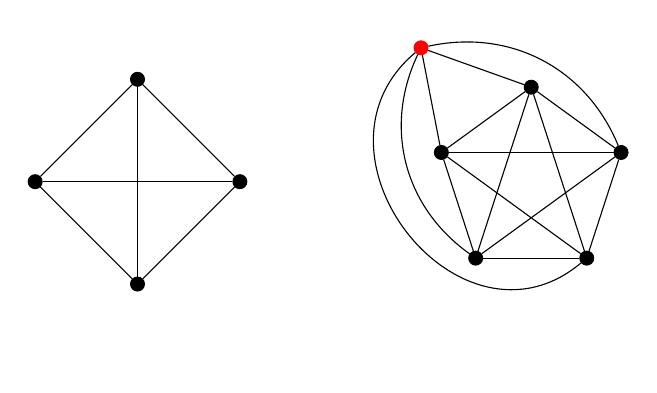
\begin{tikzpicture}[
    mycircle/.style={
        circle,
        draw=black,
        fill=black,
        fill opacity = 1,
        inner sep=0pt,
        minimum size=5pt,
        font=\small},
    nocircle/.style={
        circle,
        draw=black,
        fill=black,
        fill opacity = 1,
        inner sep=0pt,
        minimum size=0.45pt,
        font=\small},
    targetcircle/.style={
        circle,
        draw=red,
        fill=red,
        fill opacity = 1,
        inner sep=0pt,
        minimum size=5pt,
        font=\small},
    myarrow/.style={-},
    dottedarrow/.style={-,dashed},
    thiccarrow/.style={-,line width=0.9pt},
    node distance=1.2cm and 1.5cm
]


\begin{scope}
    \begin{scope}[rotate=90]
        \foreach \x/\y in {0/a,90/b,180/c, 270/d}{ % color in outer layer
        \node[mycircle] (\y) at (canvas polar cs: radius=1.3cm,angle=\x){};
        }
    \end{scope}

    \path[every node/.style={font=\sffamily\small}]
        (a) edge [color=black] (b)
        (a) edge [color=black] (c)
        (a) edge [color=black] (d)
        (b) edge [color=black] (c)
        (b) edge [color=black] (d)
        (c) edge [color=black] (d);
\end{scope}

\begin{scope}[xshift=5cm]
    \begin{scope}[rotate=90]
        \foreach \x/\y in {0/0,72/1,144/2, 216/3, 288/4}{ % color in outer layer
        \node[mycircle] (\y) at (canvas polar cs: radius=1.2cm,angle=\x){};
        }
    \end{scope}

    \path[every node/.style={font=\sffamily\small}]
        (0) edge [color=black] (1)
        (0) edge [color=black] (2)
        (0) edge [color=black] (3)
        (0) edge [color=black] (4)
        (1) edge [color=black] (2)
        (1) edge [color=black] (3)
        (1) edge [color=black] (4)
        (2) edge [color=black] (3)
        (2) edge [color=black] (4)
        (3) edge [color=black] (4);

    \node[targetcircle] (x) at (-1.4, 1.7) {};

    \path[every node/.style={font=\sffamily\small}]
        (x) edge [color=black] (0)
        (x) edge [color=black] (1)
        (x) edge [color=black, bend right=40] (2)
        (x) edge [color=black, out=220, in=-140, looseness=1.5] (3)
        (x) edge [color=black, bend left=40] (4);
\end{scope}
\end{tikzpicture}
\end{document}}
            \caption{Simplification of the 2 Community network at $t=1$.}
        \end{subfigure}
        \hfill
        \centering
        \begin{subfigure}[c]{0.3\textwidth}
            \centering
            \resizebox{.6\width}{!}{\documentclass{standalone}
\usepackage{amsmath,amssymb,amsthm}
\usepackage{tikz}
\usetikzlibrary{decorations.markings}
\usetikzlibrary{arrows,automata}
\usetikzlibrary{positioning}
\usetikzlibrary{arrows.meta,positioning}

\begin{document}
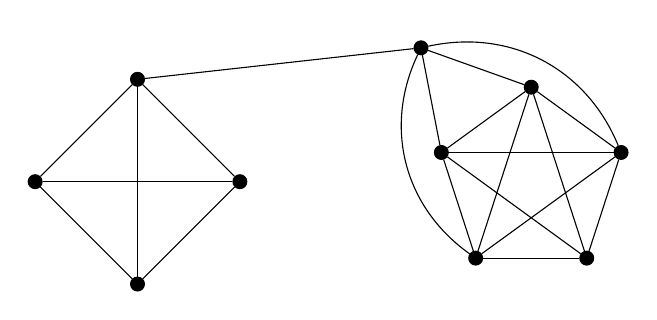
\begin{tikzpicture}[
    mycircle/.style={
        circle,
        draw=black,
        fill=black,
        fill opacity = 1,
        inner sep=0pt,
        minimum size=5pt,
        font=\small},
    nocircle/.style={
        circle,
        draw=black,
        fill=black,
        fill opacity = 1,
        inner sep=0pt,
        minimum size=0.45pt,
        font=\small},
    myarrow/.style={-},
    dottedarrow/.style={-,dashed},
    thiccarrow/.style={-,line width=0.9pt},
    node distance=1.2cm and 1.5cm
]
\begin{scope}
    \begin{scope}[rotate=90]
        \foreach \x/\y in {0/a,90/b,180/c, 270/d}{ % color in outer layer
        \node[mycircle] (\y) at (canvas polar cs: radius=1.3cm,angle=\x){};
        }
    \end{scope}

    \path[every node/.style={font=\sffamily\small}]
        (a) edge [color=black] (b)
        (a) edge [color=black] (c)
        (a) edge [color=black] (d)
        (b) edge [color=black] (c)
        (b) edge [color=black] (d)
        (c) edge [color=black] (d);
\end{scope}

\begin{scope}[xshift=5cm]
    \begin{scope}[rotate=90]
        \foreach \x/\y in {0/0,72/1,144/2, 216/3, 288/4}{ % color in outer layer
        \node[mycircle] (\y) at (canvas polar cs: radius=1.2cm,angle=\x){};
        }
    \end{scope}

    \path[every node/.style={font=\sffamily\small}]
        (0) edge [color=black] (1)
        (0) edge [color=black] (2)
        (0) edge [color=black] (3)
        (0) edge [color=black] (4)
        (1) edge [color=black] (2)
        (1) edge [color=black] (3)
        (1) edge [color=black] (4)
        (2) edge [color=black] (3)
        (2) edge [color=black] (4)
        (3) edge [color=black] (4);

    \node[mycircle] (x) at (-1.4, 1.7) {};

    \path[every node/.style={font=\sffamily\small}]
        (x) edge [color=black] (0)
        (x) edge [color=black] (1)
        (x) edge [color=black, bend right=40] (2)
        (x) edge [color=black, bend left=40] (4)
        (x) edge [color=black] (a);
\end{scope}
\end{tikzpicture}
\end{document}}
            \caption{Simplification of the 2 Community network at $t=2$.}
        \end{subfigure}
        \hfill
        \centering
        \begin{subfigure}[c]{0.3\textwidth}
            \centering
            \resizebox{.6\width}{!}{\documentclass{standalone}
\usepackage{amsmath,amssymb,amsthm}
\usepackage{tikz}
\usetikzlibrary{decorations.markings}
\usetikzlibrary{arrows,automata}
\usetikzlibrary{positioning}
\usetikzlibrary{arrows.meta,positioning}

\begin{document}
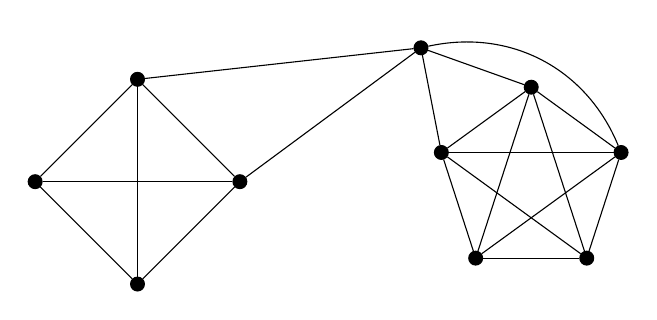
\begin{tikzpicture}[
    mycircle/.style={
        circle,
        draw=black,
        fill=black,
        fill opacity = 1,
        inner sep=0pt,
        minimum size=5pt,
        font=\small},
    nocircle/.style={
        circle,
        draw=black,
        fill=black,
        fill opacity = 1,
        inner sep=0pt,
        minimum size=0.45pt,
        font=\small},
    myarrow/.style={-},
    dottedarrow/.style={-,dashed},
    thiccarrow/.style={-,line width=0.9pt},
    node distance=1.2cm and 1.5cm
]
\begin{scope}
    \begin{scope}[rotate=90]
        \foreach \x/\y in {0/a,90/b,180/c, 270/d}{ % color in outer layer
        \node[mycircle] (\y) at (canvas polar cs: radius=1.3cm,angle=\x){};
        }
    \end{scope}

    \path[every node/.style={font=\sffamily\small}]
        (a) edge [color=black] (b)
        (a) edge [color=black] (c)
        (a) edge [color=black] (d)
        (b) edge [color=black] (c)
        (b) edge [color=black] (d)
        (c) edge [color=black] (d);
\end{scope}

\begin{scope}[xshift=5cm]
    \begin{scope}[rotate=90]
        \foreach \x/\y in {0/0,72/1,144/2, 216/3, 288/4}{ % color in outer layer
        \node[mycircle] (\y) at (canvas polar cs: radius=1.2cm,angle=\x){};
        }
    \end{scope}

    \path[every node/.style={font=\sffamily\small}]
        (0) edge [color=black] (1)
        (0) edge [color=black] (2)
        (0) edge [color=black] (3)
        (0) edge [color=black] (4)
        (1) edge [color=black] (2)
        (1) edge [color=black] (3)
        (1) edge [color=black] (4)
        (2) edge [color=black] (3)
        (2) edge [color=black] (4)
        (3) edge [color=black] (4);

    \node[mycircle] (x) at (-1.4, 1.7) {};

    \path[every node/.style={font=\sffamily\small}]
        (x) edge [color=black] (0)
        (x) edge [color=black] (1)
        (x) edge [color=black, bend left=40] (4)
        (x) edge [color=black] (a)
        (x) edge [color=black] (d);
\end{scope}
\end{tikzpicture}
\end{document}}
            \caption{Simplification of the 2 Community network at $t=3$.}
        \end{subfigure}
        \caption{First 3 time steps of synthetic 2 community network.}
        \label{2community train series}
    \end{figure}

    For the long tail network we have a large (50 nodes) fully connected component at one end. This is used to orient the embedding and model. The target node starts attatched to the node that is attatched to this large componet. At each time step the target node move one node further down the tail.
    \begin{figure}[H]
        \centering
        \begin{subfigure}[c]{0.3\textwidth}
            \centering
            \resizebox{.6\width}{!}{\documentclass{standalone}
\usepackage{amsmath,amssymb,amsthm}
\usepackage{tikz}
\usetikzlibrary{decorations.markings}
\usetikzlibrary{arrows,automata}
\usetikzlibrary{positioning}
\usetikzlibrary{arrows.meta,positioning}

\begin{document}
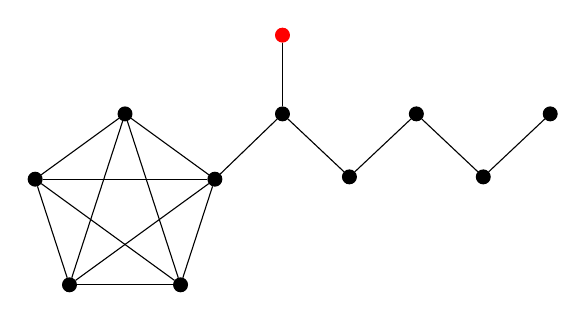
\begin{tikzpicture}[
    mycircle/.style={
        circle,
        draw=black,
        fill=black,
        fill opacity = 1,
        inner sep=0pt,
        minimum size=5pt,
        font=\small},
    nocircle/.style={
        circle,
        draw=black,
        fill=black,
        fill opacity = 1,
        inner sep=0pt,
        minimum size=0.45pt,
        font=\small},
    targetcircle/.style={
        circle,
        draw=red,
        fill=red,
        fill opacity = 1,
        inner sep=0pt,
        minimum size=5pt,
        font=\small},
    myarrow/.style={-},
    dottedarrow/.style={-,dashed},
    thiccarrow/.style={-,line width=0.9pt},
    node distance=1.2cm and 1.5cm
]
\begin{scope}
    \begin{scope}[rotate=90]
        \foreach \x/\y in {0/0,72/1,144/2, 216/3, 288/4}{ % color in outer layer
        \node[mycircle] (\y) at (canvas polar cs: radius=1.2cm,angle=\x){};
        }
    \end{scope}

    \path[every node/.style={font=\sffamily\small}]
        (0) edge [color=black] (1)
        (0) edge [color=black] (2)
        (0) edge [color=black] (3)
        (0) edge [color=black] (4)
        (1) edge [color=black] (2)
        (1) edge [color=black] (3)
        (1) edge [color=black] (4)
        (2) edge [color=black] (3)
        (2) edge [color=black] (4)
        (3) edge [color=black] (4);

    \node[mycircle] (a) at (2, 1.2) {};
    \node[mycircle] (b) at (2.85, 0.4) {};
    \node[mycircle] (c) at (3.7, 1.2) {};
    \node[mycircle] (d) at (4.55, 0.4) {};
    \node[mycircle] (e) at (5.4, 1.2) {};

    \path[every node/.style={font=\sffamily\small}]
        (4) edge [color=black] (a)
        (a) edge [color=black] (b)
        (b) edge [color=black] (c)
        (c) edge [color=black] (d)
        (d) edge [color=black] (e);

    \node[targetcircle] (x) at (2, 2.2) {};

    \path[every node/.style={font=\sffamily\small}]
        (x) edge [color=black] (a);
\end{scope}
\end{tikzpicture}
\end{document}}
            \caption{Simplification of the long tail network at $t=1$.}
        \end{subfigure}
        \hfill
        \centering
        \begin{subfigure}[c]{0.3\textwidth}
            \centering
            \resizebox{.6\width}{!}{\documentclass{standalone}
\usepackage{amsmath,amssymb,amsthm}
\usepackage{tikz}
\usetikzlibrary{decorations.markings}
\usetikzlibrary{arrows,automata}
\usetikzlibrary{positioning}
\usetikzlibrary{arrows.meta,positioning}

\begin{document}
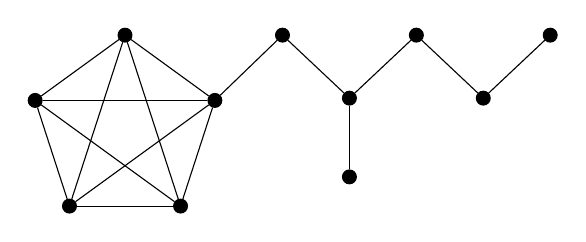
\begin{tikzpicture}[
    mycircle/.style={
        circle,
        draw=black,
        fill=black,
        fill opacity = 1,
        inner sep=0pt,
        minimum size=5pt,
        font=\small},
    nocircle/.style={
        circle,
        draw=black,
        fill=black,
        fill opacity = 1,
        inner sep=0pt,
        minimum size=0.45pt,
        font=\small},
    myarrow/.style={-},
    dottedarrow/.style={-,dashed},
    thiccarrow/.style={-,line width=0.9pt},
    node distance=1.2cm and 1.5cm
]

\begin{scope}
    \begin{scope}[rotate=90]
        \foreach \x/\y in {0/0,72/1,144/2, 216/3, 288/4}{ % color in outer layer
        \node[mycircle] (\y) at (canvas polar cs: radius=1.2cm,angle=\x){};
        }
    \end{scope}

    \path[every node/.style={font=\sffamily\small}]
        (0) edge [color=black] (1)
        (0) edge [color=black] (2)
        (0) edge [color=black] (3)
        (0) edge [color=black] (4)
        (1) edge [color=black] (2)
        (1) edge [color=black] (3)
        (1) edge [color=black] (4)
        (2) edge [color=black] (3)
        (2) edge [color=black] (4)
        (3) edge [color=black] (4);

    \node[mycircle] (a) at (2, 1.2) {};
    \node[mycircle] (b) at (2.85, 0.4) {};
    \node[mycircle] (c) at (3.7, 1.2) {};
    \node[mycircle] (d) at (4.55, 0.4) {};
    \node[mycircle] (e) at (5.4, 1.2) {};

    \path[every node/.style={font=\sffamily\small}]
        (4) edge [color=black] (a)
        (a) edge [color=black] (b)
        (b) edge [color=black] (c)
        (c) edge [color=black] (d)
        (d) edge [color=black] (e);

    \node[mycircle] (x) at (2.85, -0.6) {};

    \path[every node/.style={font=\sffamily\small}]
        (x) edge [color=black] (b);
\end{scope}
\end{tikzpicture}
\end{document}}
            \caption{Simplification of the long tail network at $t=2$.}
        \end{subfigure}
        \hfill
        \centering
        \begin{subfigure}[c]{0.3\textwidth}
            \centering
            \resizebox{.6\width}{!}{\documentclass{standalone}
\usepackage{amsmath,amssymb,amsthm}
\usepackage{tikz}
\usetikzlibrary{decorations.markings}
\usetikzlibrary{arrows,automata}
\usetikzlibrary{positioning}
\usetikzlibrary{arrows.meta,positioning}

\begin{document}
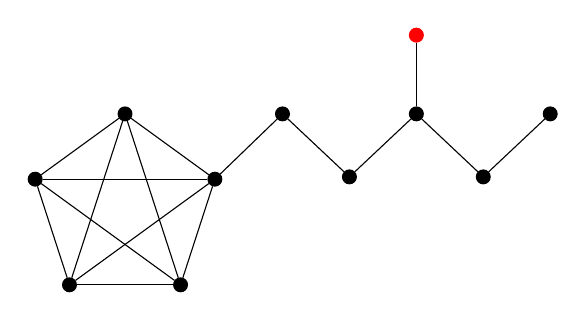
\begin{tikzpicture}[
    mycircle/.style={
        circle,
        draw=black,
        fill=black,
        fill opacity = 1,
        inner sep=0pt,
        minimum size=5pt,
        font=\small},
    nocircle/.style={
        circle,
        draw=black,
        fill=black,
        fill opacity = 1,
        inner sep=0pt,
        minimum size=0.45pt,
        font=\small},
    targetcircle/.style={
        circle,
        draw=red,
        fill=red,
        fill opacity = 1,
        inner sep=0pt,
        minimum size=5pt,
        font=\small},
    myarrow/.style={-},
    dottedarrow/.style={-,dashed},
    thiccarrow/.style={-,line width=0.9pt},
    node distance=1.2cm and 1.5cm
]

\begin{scope}
    \begin{scope}[rotate=90]
        \foreach \x/\y in {0/0,72/1,144/2, 216/3, 288/4}{ % color in outer layer
        \node[mycircle] (\y) at (canvas polar cs: radius=1.2cm,angle=\x){};
        }
    \end{scope}

    \path[every node/.style={font=\sffamily\small}]
        (0) edge [color=black] (1)
        (0) edge [color=black] (2)
        (0) edge [color=black] (3)
        (0) edge [color=black] (4)
        (1) edge [color=black] (2)
        (1) edge [color=black] (3)
        (1) edge [color=black] (4)
        (2) edge [color=black] (3)
        (2) edge [color=black] (4)
        (3) edge [color=black] (4);

    \node[mycircle] (a) at (2, 1.2) {};
    \node[mycircle] (b) at (2.85, 0.4) {};
    \node[mycircle] (c) at (3.7, 1.2) {};
    \node[mycircle] (d) at (4.55, 0.4) {};
    \node[mycircle] (e) at (5.4, 1.2) {};

    \path[every node/.style={font=\sffamily\small}]
        (4) edge [color=black] (a)
        (a) edge [color=black] (b)
        (b) edge [color=black] (c)
        (c) edge [color=black] (d)
        (d) edge [color=black] (e);

    \node[targetcircle] (x) at (3.7, 2.2) {};

    \path[every node/.style={font=\sffamily\small}]
        (x) edge [color=black] (c);
\end{scope}
\end{tikzpicture}
\end{document}}
            \caption{Simplification of the long tail network at $t=3$.}
        \end{subfigure}\\
        \caption{First 3 time steps of synthetic long tail network.}
    \end{figure}    


    We also create a set of three communities. The target node starts connected to all of these communities with each community having a different number of edges. The community with the fewest edges between the target node will have one edge removed at each timestep. The communities have sizes 40, 35, 30 and have 25, 24, and 23 edges to the target node respectively. 
    \begin{figure}[H]
        \centering
        \centering
        \begin{subfigure}[c]{0.3\textwidth}
            \centering
            \resizebox{.6\width}{!}{\documentclass{standalone}
\usepackage{amsmath,amssymb,amsthm}
\usepackage{tikz}
\usetikzlibrary{decorations.markings}
\usetikzlibrary{arrows,automata}
\usetikzlibrary{positioning}
\usetikzlibrary{arrows.meta,positioning}

\begin{document}
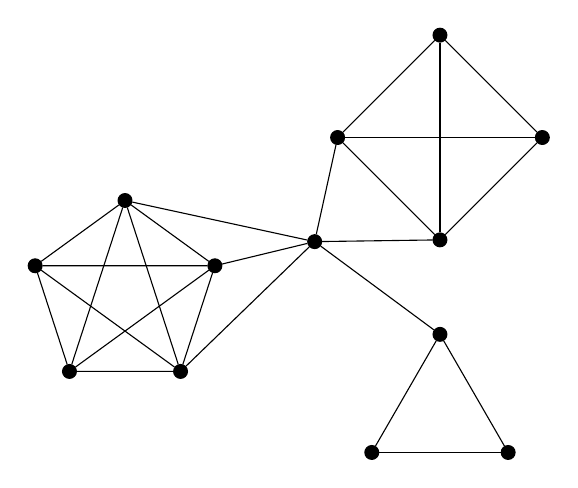
\begin{tikzpicture}[
    mycircle/.style={
        circle,
        draw=black,
        fill=black,
        fill opacity = 1,
        inner sep=0pt,
        minimum size=5pt,
        font=\small},
    nocircle/.style={
        circle,
        draw=black,
        fill=black,
        fill opacity = 1,
        inner sep=0pt,
        minimum size=0.45pt,
        font=\small},
    myarrow/.style={-},
    dottedarrow/.style={-,dashed},
    thiccarrow/.style={-,line width=0.9pt},
    node distance=1.2cm and 1.5cm
]
\begin{scope}
    \begin{scope}[rotate=-90]
        \foreach \x/\y in {0/a,90/b,180/c, 270/d}{ % color in outer layer
        \node[mycircle] (\y) at (canvas polar cs: radius=1.3cm,angle=\x){};
        }
    \end{scope}

    \path[every node/.style={font=\sffamily\small}]
        (a) edge [color=black] (b)
        (a) edge [color=black] (c)
        (a) edge [color=black] (d)
        (b) edge [color=black] (c)
        (b) edge [color=black] (d)
        (c) edge [color=black] (d);
\end{scope}

\begin{scope}[xshift=-4cm, yshift=-2cm, rotate=-72]
    \begin{scope}[rotate=90]
        \foreach \x/\y in {0/0,72/1,144/2, 216/3, 288/4}{ % color in outer layer
        \node[mycircle] (\y) at (canvas polar cs: radius=1.2cm,angle=\x){};
        }
    \end{scope}

    \path[every node/.style={font=\sffamily\small}]
        (0) edge [color=black] (1)
        (0) edge [color=black] (2)
        (0) edge [color=black] (3)
        (0) edge [color=black] (4)
        (1) edge [color=black] (2)
        (1) edge [color=black] (3)
        (1) edge [color=black] (4)
        (2) edge [color=black] (3)
        (2) edge [color=black] (4)
        (3) edge [color=black] (4);

    \node[mycircle] (x) at (0.1, 2.5) {};

    \path[every node/.style={font=\sffamily\small}]
        (x) edge [color=black] (0)
        (x) edge [color=black] (1)
        (x) edge [color=black] (4)
        (x) edge [color=black] (a)
        (x) edge [color=black] (d);
\end{scope}

\begin{scope}[yshift=-3.5cm, xshift=0cm]
    \begin{scope}[rotate=90]
        \foreach \x/\y in {0/0,120/1,240/2}{ % color in outer layer
        \node[mycircle] (\y) at (canvas polar cs: radius=1cm,angle=\x){};
        }
    \end{scope}

    \path[every node/.style={font=\sffamily\small}]
        (0) edge [color=black] (1)
        (0) edge [color=black] (2)
        (1) edge [color=black] (2)
        (x) edge [color=black] (0);
\end{scope}
\end{tikzpicture}
\end{document}}
            \caption{Simplification of the 3 Community network at $t=1$.}
        \end{subfigure}
        \hfill
        \centering
        \begin{subfigure}[c]{0.3\textwidth}
            \centering
            \resizebox{.6\width}{!}{\documentclass{standalone}
\usepackage{amsmath,amssymb,amsthm}
\usepackage{tikz}
\usetikzlibrary{decorations.markings}
\usetikzlibrary{arrows,automata}
\usetikzlibrary{positioning}
\usetikzlibrary{arrows.meta,positioning}

\begin{document}
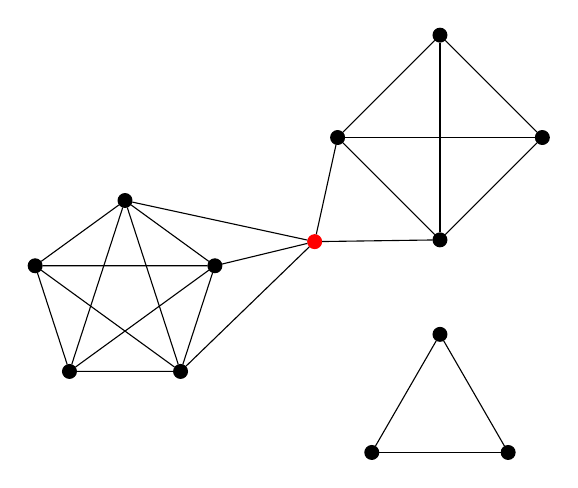
\begin{tikzpicture}[
    mycircle/.style={
        circle,
        draw=black,
        fill=black,
        fill opacity = 1,
        inner sep=0pt,
        minimum size=5pt,
        font=\small},
    nocircle/.style={
        circle,
        draw=black,
        fill=black,
        fill opacity = 1,
        inner sep=0pt,
        minimum size=0.45pt,
        font=\small},
    targetcircle/.style={
        circle,
        draw=red,
        fill=red,
        fill opacity = 1,
        inner sep=0pt,
        minimum size=5pt,
        font=\small},
    myarrow/.style={-},
    dottedarrow/.style={-,dashed},
    thiccarrow/.style={-,line width=0.9pt},
    node distance=1.2cm and 1.5cm
]
\begin{scope}
    \begin{scope}[rotate=-90]
        \foreach \x/\y in {0/a,90/b,180/c, 270/d}{ % color in outer layer
        \node[mycircle] (\y) at (canvas polar cs: radius=1.3cm,angle=\x){};
        }
    \end{scope}

    \path[every node/.style={font=\sffamily\small}]
        (a) edge [color=black] (b)
        (a) edge [color=black] (c)
        (a) edge [color=black] (d)
        (b) edge [color=black] (c)
        (b) edge [color=black] (d)
        (c) edge [color=black] (d);
\end{scope}

\begin{scope}[xshift=-4cm, yshift=-2cm, rotate=-72]
    \begin{scope}[rotate=90]
        \foreach \x/\y in {0/0,72/1,144/2, 216/3, 288/4}{ % color in outer layer
        \node[mycircle] (\y) at (canvas polar cs: radius=1.2cm,angle=\x){};
        }
    \end{scope}

    \path[every node/.style={font=\sffamily\small}]
        (0) edge [color=black] (1)
        (0) edge [color=black] (2)
        (0) edge [color=black] (3)
        (0) edge [color=black] (4)
        (1) edge [color=black] (2)
        (1) edge [color=black] (3)
        (1) edge [color=black] (4)
        (2) edge [color=black] (3)
        (2) edge [color=black] (4)
        (3) edge [color=black] (4);

    \node[targetcircle] (x) at (0.1, 2.5) {};

    \path[every node/.style={font=\sffamily\small}]
        (x) edge [color=black] (0)
        (x) edge [color=black] (1)
        (x) edge [color=black] (4)
        (x) edge [color=black] (a)
        (x) edge [color=black] (d);
\end{scope}

\begin{scope}[yshift=-3.5cm, xshift=0cm]
    \begin{scope}[rotate=90]
        \foreach \x/\y in {0/0,120/1,240/2}{ % color in outer layer
        \node[mycircle] (\y) at (canvas polar cs: radius=1cm,angle=\x){};
        }
    \end{scope}

    \path[every node/.style={font=\sffamily\small}]
        (0) edge [color=black] (1)
        (0) edge [color=black] (2)
        (1) edge [color=black] (2);
\end{scope}
\end{tikzpicture}
\end{document}}
            \caption{Simplification of the 3 Community network at $t=2$.}
        \end{subfigure}
        \hfill
        \centering
        \begin{subfigure}[c]{0.3\textwidth}
            \centering
            \resizebox{.6\width}{!}{\documentclass{standalone}
\usepackage{amsmath,amssymb,amsthm}
\usepackage{tikz}
\usetikzlibrary{decorations.markings}
\usetikzlibrary{arrows,automata}
\usetikzlibrary{positioning}
\usetikzlibrary{arrows.meta,positioning}

\begin{document}
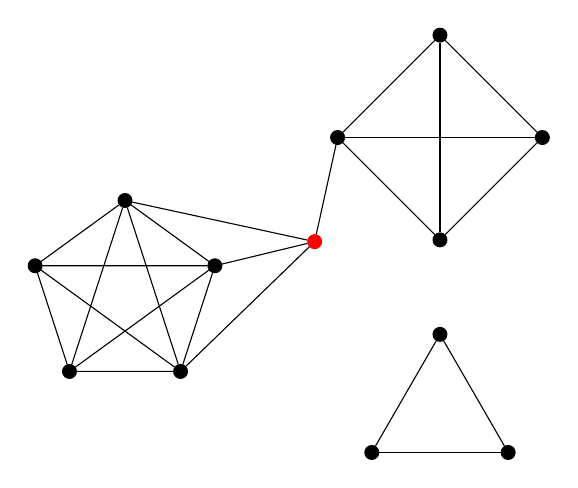
\begin{tikzpicture}[
    mycircle/.style={
        circle,
        draw=black,
        fill=black,
        fill opacity = 1,
        inner sep=0pt,
        minimum size=5pt,
        font=\small},
    nocircle/.style={
        circle,
        draw=black,
        fill=black,
        fill opacity = 1,
        inner sep=0pt,
        minimum size=0.45pt,
        font=\small},
    targetcircle/.style={
        circle,
        draw=red,
        fill=red,
        fill opacity = 1,
        inner sep=0pt,
        minimum size=5pt,
        font=\small},
    myarrow/.style={-},
    dottedarrow/.style={-,dashed},
    thiccarrow/.style={-,line width=0.9pt},
    node distance=1.2cm and 1.5cm
]
\begin{scope}
    \begin{scope}[rotate=-90]
        \foreach \x/\y in {0/a,90/b,180/c, 270/d}{ % color in outer layer
        \node[mycircle] (\y) at (canvas polar cs: radius=1.3cm,angle=\x){};
        }
    \end{scope}

    \path[every node/.style={font=\sffamily\small}]
        (a) edge [color=black] (b)
        (a) edge [color=black] (c)
        (a) edge [color=black] (d)
        (b) edge [color=black] (c)
        (b) edge [color=black] (d)
        (c) edge [color=black] (d);
\end{scope}

\begin{scope}[xshift=-4cm, yshift=-2cm, rotate=-72]
    \begin{scope}[rotate=90]
        \foreach \x/\y in {0/0,72/1,144/2, 216/3, 288/4}{ % color in outer layer
        \node[mycircle] (\y) at (canvas polar cs: radius=1.2cm,angle=\x){};
        }
    \end{scope}

    \path[every node/.style={font=\sffamily\small}]
        (0) edge [color=black] (1)
        (0) edge [color=black] (2)
        (0) edge [color=black] (3)
        (0) edge [color=black] (4)
        (1) edge [color=black] (2)
        (1) edge [color=black] (3)
        (1) edge [color=black] (4)
        (2) edge [color=black] (3)
        (2) edge [color=black] (4)
        (3) edge [color=black] (4);

    \node[targetcircle] (x) at (0.1, 2.5) {};

    \path[every node/.style={font=\sffamily\small}]
        (x) edge [color=black] (0)
        (x) edge [color=black] (1)
        (x) edge [color=black] (4)
        (x) edge [color=black] (d);
\end{scope}

\begin{scope}[yshift=-3.5cm, xshift=0cm]
    \begin{scope}[rotate=90]
        \foreach \x/\y in {0/0,120/1,240/2}{ % color in outer layer
        \node[mycircle] (\y) at (canvas polar cs: radius=1cm,angle=\x){};
        }
    \end{scope}

    \path[every node/.style={font=\sffamily\small}]
        (0) edge [color=black] (1)
        (0) edge [color=black] (2)
        (1) edge [color=black] (2);
\end{scope}
\end{tikzpicture}
\end{document}}
            \caption{Simplification of the 3 Community network at $t=3$.}
        \end{subfigure}
        \caption{First 3 time steps of synthetic 3 community network.}
        \label{3community train series}
    \end{figure}
    The 2 community temporal network was selected to illustrate that this process can be used to model a node changing communities in ideal conditions, and the long tail network was selected because we wanted to present these models with a range of problems. The two community problem is difficult for the neural network to learn because the same set of distances as input need to result in different outputs. The long tail problem is difficult for the embedding because a large portion of the network is along the off diagonals; meaning that, to get an accurate embedding, the dimension of the embedding would need to be close to the length of the tail. The three community problem should be the easiest to solve because it has been dileberately constructed to avoid the problems the other two models face.

\end{section}
\begin{section}{Results}
    For each of theses systems, we took embedded the temporal network in two dimensions at each time step. The temporal embeddings were then divided into a training set of 20 and a testing set of 15. The output of the trained neural networks was then used to train a symbolic regression model that could use a simple set of addition, subtraction, division, and multiplication. 

    \begin{subsection}{2 Community}
        \begin{figure}
            \foreach \i in {1,...,15} {%
                \begin{subfigure}[p]{0.3\textwidth}
                    \includegraphics[width=\linewidth]{/home/stirling/thesis/Conference Submission/Plots/Test Only/2communities/2communities \i.png}
                    \caption{t=\i}
                \end{subfigure}\quad
            }
            \caption{2 Community test series. This series shows the comparison of the neural network model, the symbolic regression model trained on the neural network model, and the true solution of the two community system.}
            \label{2community series}
        \end{figure}
        In fig \ref{2community series} the green points are the embedded coordinates of the node in each of the communities. Each cluster is one separate community. The orange point is the true coordinate of the embedded target node at each time step. The blue point is our model prediction from the true target node at the first time step. As the time progresses, we see the true node move from one community cluster to the other. This is expected from the embedding; the target node starts as very similar to the first community (as it has many connections with nodes in that community) and as time progresses, it gradually becomes less and less similar to the first community and more similar to the second (as the edges between the target node and the first community are replaced with edges to the second community). As such, we see the target node move towards the second community.

        In this case we see the symbolic regression overshoot the location of the target node and move far ahead of its location by the end of the training data. In contrast, the neural network moves away from the target node at first, then maintain that distance throughout the training data. This system was set up and trained multiple times, and each time we saw the symbolic regression model behave more erratically than the neural network model predictions.
    \end{subsection}

    \begin{subsection}{Long Tail}
        \begin{figure}
            \foreach \i in {1,...,15} {%
                \begin{subfigure}[p]{0.3\textwidth}
                    \includegraphics[width=\linewidth]{/home/stirling/thesis/Conference Submission/Plots/Test Only/longTail/longTail \i.png}
                    \caption{t=\i}
                \end{subfigure}\quad
            }
            \caption{3 Community test series. This series shows the comparison of the neural network model, the symbolic regression model trained on the neural network model, and the true solution of the long tail system.}
            \label{longtail series}
        \end{figure}
        In fig \ref{longtail series} we see the true embedding of the target node jump from one arm to the other at each timestep. It is clear that neither the the symbolic regression model nor the neural network model capture this movement, but the symbolic regression model does not move away from the data as quickly as the neural network model does.

        In contrast to this, the symbolic regression model remains close to the true target node throughout the test data.       
    \end{subsection}

    \begin{subsection}{Three Community (Please Review)}
        \begin{figure}
            \foreach \i in {1,...,15} {%
                \begin{subfigure}[p]{0.3\textwidth}
                    \includegraphics[width=\linewidth]{/home/stirling/thesis/Conference Submission/Plots/Test Only/3community/3community \i.png}
                    \caption{t=\i}
                \end{subfigure}\quad
            }
            \caption{Long tail test series. This series shows the comparison of the neural network model, the symbolic regression model trained on the neural network model, and the true solution of the 3 community system.}
            \label{3community series}
        \end{figure}
        In fig \ref{3community series} we again, as the edges between the community with the fewest edges are removed, we see the target node move away from it in the embedding and towards the other two clusters of points (communities).

        In the neural network only model, we see the prediction follow the true target node very closely at first. We then see the node drift further and further from the true target node. In contrast, the symbolic regression model remains much closer to the true position of the target node as the test data progresses. We see the symbolic regression move slightly ahead of the true location at first, but this distance remains relatively constant thereafter.
    \end{subsection}

\end{section}

\begin{section}{Discussion}
    \begin{subsection}{Two Community}
        It is interesting to see the symbolic regression model perform so much more poorly than the neural network model in this system. When we view the training section of the data, we see that there is a downward curve in the neural network predictions towards the end of the training data. It seems that the symbolic regression model picked this up and continued the downward trajectory throughout the test data. This downward curve may be because the problem that we are trying to solve is symmetrical. That is the same set of distances as input into the neural network, the target node needs to move away from its nearest neighbours in the first half, then move towards its nearest neighbours in the second half. Potential ways of breaking this symmetry may be to include information of the previous timestep, or to include the absolute position of the target node as input into the neural network. 

    \end{subsection}

    \begin{subsection}{Long Tail}
        We see that neither the neural network model capture the movement of the target node to any real extent. One reason for this may again be an issue of symmetrical input. The distances from the k nearest neighbours to the target node do not seem to change much as the target node jumps from one arm to the other, but the neural network somehow needs to learn to jump left then right at alternating timesteps. The solutions to this would be the same as for the two community system.
    \end{subsection}
    \begin{subsection}{Three Community}
        This was by far the largest improvement between the neural network and the symbolic regression. This could be because this system had the least difference between the training predictions and the true position of the target node. At the end of the test data we see the true target node move towards the origin. This is because it now only has edges to one community and so at each timestep it removes one of these. If this had continued, the target node would have no edges. Nodes with no edges are mapped to the origin. When this happened, the symbolic regression model prediction began to move further from the true node.

        We see a large difference in the training predictions between the 2 and 3 community systems. In the 2 community system, even in the training period, the predictions tended to wander and be less accurate. Whereas the 3 community training predictions remained very close to the true target node. The movement of the target node in the embedding was very similar between the two systems, and so the difference seems to be that the 2 community has symmetrical inputs.
    \end{subsection}
    Using symbolic regression to approximate the neural network output seems to increase the stability of the extrapolation. This is most pronounced 

\begin{section}{Conclusion}
    Not sure what to write for this
\end{section}
\end{section}


% \begin{section}{What Next?}
%     - optimisation\\
%     - Scale up\\
%     - Include more structural knowledge with underlying\\
%     - Find and use real world data to test against
% \end{section}
\printbibliography

\end{document}

% draft for miguel
% all absolute pos of nodes
% polar positions

% questions for Giulio:
%     Why both NN and sym reg not just sym reg
%     Why cos dist